\begin{figure}[h!]
\centering
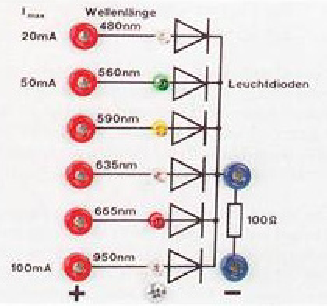
\includegraphics[scale=1]{Grafiken/Schaltplatte.pdf}
\caption{Das Schaltbrett mit den Leuchtdioden \cite{Metzler07}}
\end{figure}
An einem Schaltbrett sind Leuchtdioden mit verschiedenen Wellenlängen angebracht. Fünf dieser Dioden werden vermessen. Sie werden nach einander an eine Konstantstromquelle angeschlossen und parallel zur Diode wird eine Spannungsmessgerät angeschlossen. Nun werden Strom- und Spannungswertepaare aufgenommen.

